\section{Dipendenza della frequenza dal numero di armonica}

Nella prima parte dell'esperienza è stata studiata la formazione delle onde stazionarie su una corda vibrante mantenendo costante la lunghezza e la tensione ad essa applicata, variando la frequenza della forzante esterna.  
La lunghezza della corda è stata misurata con un metro a nastro, ottenendo $L = \qty{2.487 \pm 0.015}{\meter}$, mentre per il tratto vibrante utilizzato nelle misure si è ottenuto
$L_{\text{tratto}} = \qty{0.657 \pm 0.015}{\meter}$. L'incertezza sulle lunghezze è stata determinata assumendo errori di allineamento tra il metro e la strumentazione, oltre all'allungamento a cui la corda è sottoposta durante le misure.
Tramite bilancia analitica si è misurata la massa della corda, il cui valore è $m = \qty{5.2 \pm 0.5}{\gram}$ da cui si ricava la massa lineare $\mu = \frac{m}{L} = \qty{2.1 \pm 0.2}{\gram\per\meter}$. La tensione della corda è dovuta esclusivamente alla massa del supporto appeso, ossia $m_{supporto} = \qty{ 80.6 \pm 0.5}{\gram}$.\\
Sono state ricercate sperimentalmente le condizioni di risonanza corrispondenti alle prime quattro armoniche della corda vibrante. Le frequenze misurate sono riportate in Tabella 1, stimando un'incertezza pari a $\sigma_f = \qty{0.5}{\hertz}$, ottenuta come semidispersione dell'intervallo di frequenze in cui si instaurava la risonanza.

\begin{table}[H]
\centering
\begin{tabular}{ccc}
\hline
  \textbf{Ordine armonico} & \ \textbf{Frequenza} \textbf{(\unit{\hertz})} & \textbf{Incertezza} \textbf{(\unit{\hertz})}\\
\hline
1 & 16.0 & 0.5\\
2 & 32.5 & 0.5\\
3 & 48.0 & 0.5\\
4 & 63.5 & 0.5\\
\hline
\end{tabular}
\caption{Frequenze e incertezze al variare di n, numero di armonica.}
\end{table}
I dati sono stati interpolati linearmente mediante metodo dei minimi quadrati,  con un fit passante per l'origine, riportato in Figura 1.
\begin{figure}[H]
    \centering
    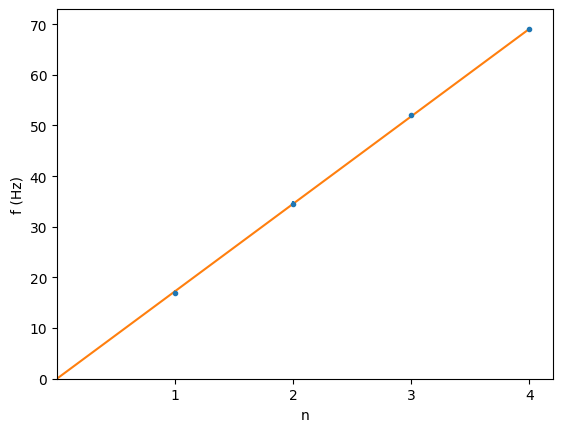
\includegraphics[width=0.6\textwidth]{Immagini/1.png}
    \caption{Interpolazione della frequenza in funzione del numero armonico con un parametro libero.}
\end{figure}

Il test del $\chi^2$ restituisce un $\Tilde{\chi}_o^2$=0.16, che per tre gradi di libertà corrisponde ad una probabilità di adattamento del 92.6\%. Si conferma perciò la dipendenza lineare tra frequenza e numero armonico, in accordo con la relazione:

\begin{equation}
  f_n = \frac{nv}{2L}
  \label{eq:frequenze}
\end{equation}

dove $n$ è il numero di armonica e $v$ la velocità di propagazione dell'onda sulla corda.
Il coefficiente angolare interpolato è $k_1 = \qty{17.27 \pm 0.09}{\hertz}$, mentre quello ricavato dalla relazione \eqref{eq:frequenze} è $k'_1 = \qty{19.0 \pm 1.0}{\hertz}$. Tramite un t-test è stata verificata la compatibilità di questi due valori, ottenendo $t_0 = 1.52$ calcolato come:
\begin{equation}
t_0 = \frac{\abs{x_1-x_2}}{\sqrt{{\sigma}_{x_1}^2+{\sigma}_{x_2}^2}}
\label{eq:t_test}
\end{equation}
 che corrisponde a una probabilità di accordo del 12.9\% tra le due misure.

 A partire da $k_1$, tramite la relazione \eqref{eq:frequenze}, si ottiene $v_1 = \qty{22.7 \pm 0.5}{\meter\per\second}$. Tale valore si può confrontare con la velocità di propagazione $v'_1 = \qty{24.7 \pm 1.2}{\meter\per\second}$, prevista dalle misure di massa lineare $\mu$ e tensione $\tau = m_{supporto}g$, tramite la relazione:

\begin{equation}
  v = \sqrt{\frac{\tau}{\mu}} 
  \label{eq:v-propagazione}
\end{equation}

Il t-test restituisce $t_0 = 1.54$, che indica una compatibilità di accordo del 12.4\%.
